\iffalse
\let\negmedspace\undefined
\let\negthickspace\undefined
\documentclass[journal,12pt,twocolumn]{IEEEtran}
\usepackage{cite}
\usepackage{amsmath,amssymb,amsfonts,amsthm}
\usepackage{algorithmic}
\usepackage{graphicx}

\usepackage{textcomp}
\usepackage{xcolor}
\usepackage{txfonts}
\usepackage{listings}
\usepackage{enumitem}
\usepackage{mathtools}
\usepackage{gensymb}
\usepackage{comment}
\usepackage[breaklinks=true]{hyperref}
\usepackage{tkz-euclide} 
\usepackage{listings}
\usepackage{gvv}                                                                      
\usepackage[latin1]{inputenc}                                
\usepackage{color}                                            
\usepackage{array}                                            
\usepackage{longtable}                                       
\usepackage{calc}                                             
\usepackage{multirow}                                         
\usepackage{hhline}                                           
\usepackage{ifthen}                                           
\usepackage{lscape}
\setlength{\arrayrulewidth}{0.5mm}
\setlength{\tabcolsep}{18pt}
\renewcommand{\arraystretch}{1.5}
\newtheorem{theorem}{Theorem}[section]
\newtheorem{problem}{Problem}
\newtheorem{proposition}{Proposition}[section]
\newtheorem{lemma}{Lemma}[section]
\newtheorem{corollary}[theorem]{Corollary}
\newtheorem{example}{Example}[section]
\newtheorem{definition}[problem]{Definition}
\newcommand{\BEQA}{\begin{eqnarray}}
\newcommand{\EEQA}{\end{eqnarray}}
\newcommand{\define}{\stackrel{\triangle}{=}}
\theoremstyle{remark}
\newtheorem{rem}{Remark}

\begin{document}

\bibliographystyle{IEEEtran}
\vspace{3cm}

\title{NCERT 12.8 8}
\author{EE23BTECH11054 - Sai Krishna Shanigarapu% <-this % stops a space
}
\maketitle
\newpage
\bigskip

\begin{flushleft}
\textbf{Question 8}\\
Suppose that the electric field amplitude of an electromagnetic wave is $E_0$ = 120N/C and that its frequency is $f$ = 50.0 MHz.\\
(a) Determine, $B_0, \omega, k$ and $\lambda$\\
(b) Find expressions for \textbf{E} and \textbf{B}\\
\end{flushleft}

\bigskip


Solution:
\fi

\begin{center}
    \begin{table}[ht]
        \caption{Input Parameters}
        \setlength{\arrayrulewidth}{0.3mm}
\setlength{\tabcolsep}{15pt}
\renewcommand{\arraystretch}{1.5}

%\textbf{Table 1}\\
\begin{center}
\begin{tabular}{ |p{1cm}|p{2.5cm}|p{1.7cm}|  }

\hline
Symbol& Description&value\\
\hline
$f$ & frequency of source & 50.0 MHz\\
\hline
$E_0$ & Electric field amplitude  & 120 N/C\\
\hline
$c$ &speed of light & 3 x 10$^8$ m/s \\
\hline
$\vec{e_2}, \vec{e_3}$ & Standard Basis vectors & N/A\\
\hline

\end{tabular}
\end{center}
        \label{tab:table1.12.8.8}
    \end{table}
\end{center}


\begin{flushleft}
    \begin{table}[ht]
       \caption{Formulae and Output}
       \setlength{\arrayrulewidth}{0.3mm}
\setlength{\tabcolsep}{15pt}
\renewcommand{\arraystretch}{1.5}

%\textbf{Table 1}\\
\begin{center}
\begin{tabular}{ |p{1cm}|p{2.5cm}|p{1.7cm}|  }

\hline
Symbol& Description&value\\
\hline
$f$ & frequency of source & 50.0 MHz\\
\hline
$E_0$ & Electric field amplitude  & 120 N/C\\
\hline
$c$ &speed of light & 3 x 10$^8$ m/s \\
\hline
$\vec{e_2}, \vec{e_3}$ & Standard Basis vectors & N/A\\
\hline

\end{tabular}
\end{center}
       \label{tab:table2.12.8.8}
    \end{table}
\bigskip
\end{flushleft}

\bigskip


\newpage
\renewcommand{\thefigure}{\theenumi}
\renewcommand{\thetable}{\theenumi}

\begin{flushleft}

\begin{figure}[h]
\renewcommand\thefigure{1}
  \caption{Graphs of $\vec{E} \text{ and } \vec{B}$}
  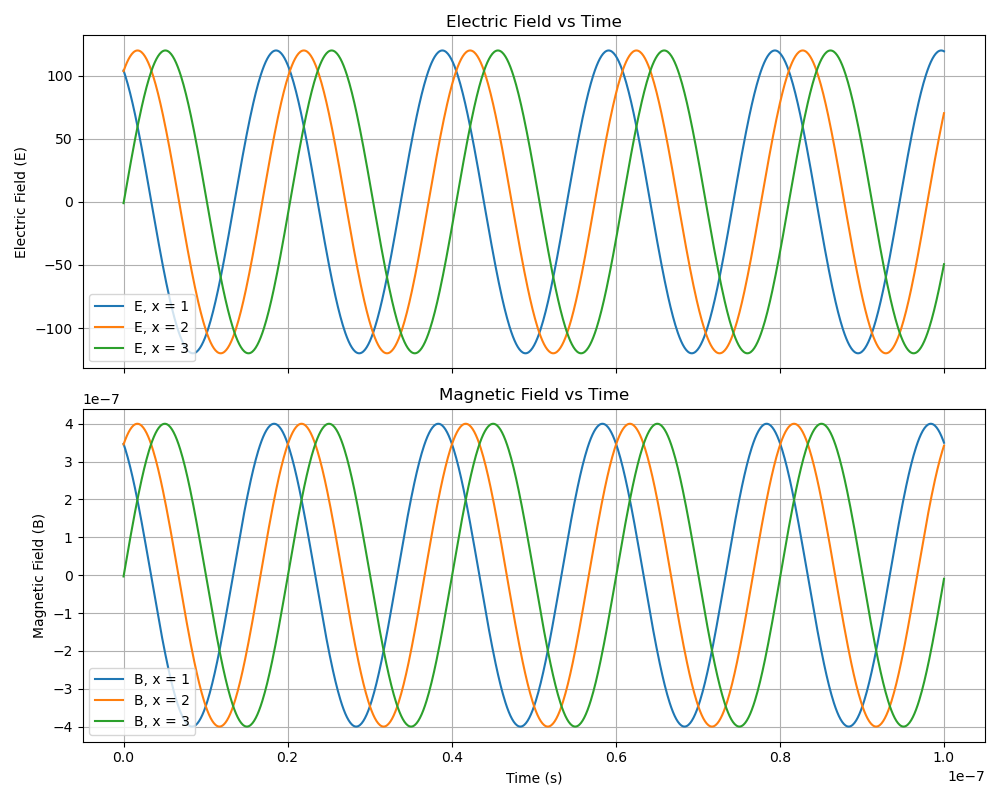
\includegraphics[width=1.05\columnwidth]{ncert-physics/12/8/8/figs/Figure_1.png}
  \label{fig:12.8.8.1}

\end{figure}

\end{flushleft}

%\end{document}
